% 知识图谱与解题流程 · ElegantNote
\documentclass[cn,11pt,color=cyan,math=newtx]{elegantnote}

% ============================================================
%  Elegant 数学教学文档 · 共享导言区
%  用法：在 \documentclass{elegantbook / elegantnote} 之后
%        % ============================================================
%  Elegant 数学教学文档 · 共享导言区
%  用法：在 \documentclass{elegantbook / elegantnote} 之后
%        % ============================================================
%  Elegant 数学教学文档 · 共享导言区
%  用法：在 \documentclass{elegantbook / elegantnote} 之后
%        \input{../common/preamble}
%  依赖：TeX Live 2026 + XeLaTeX
% ============================================================

% ---------- 等宽字体 ----------
% lmmono10 缺少 λ、≥ 等符号，改用覆盖更全的 DejaVu Sans Mono
\setmonofont{DejaVu Sans Mono}

% ---------- 数学 ----------
\usepackage{mathtools}   % amsmath 扩展（\substack、\dcases、\prescript 等）
\usepackage{bm}          % 粗体数学符号 \bm
\usepackage{cases}       % 分段函数 / 方程组 \begin{cases}
\usepackage{cancel}      % 划去 \cancel、\cancelto
\usepackage{siunitx}     % 单位与数字 \num \SI
\sisetup{
  detect-all,
  per-mode = symbol,
  range-units = single,
}

% ---------- 图形 ----------
\usepackage{tikz}
\usetikzlibrary{arrows.meta, calc, decorations.pathreplacing, positioning}
\usepackage{pgfplots}
\pgfplotsset{compat=1.18}

% ---------- 统一颜色名 ----------
% elegantbook 定义了 main / second / third；elegantnote 只有 ecolor。
% 用 \providecolor 补齐，使共享宏在两个模板下都能用。
\providecolor{main}{RGB}{0,120,2}
\providecolor{second}{RGB}{230,90,7}
\providecolor{third}{RGB}{0,160,152}

% ---------- 版式 ----------
\usepackage{fontawesome5}   % 图标（如无需要可删除本行）

% ---------- 数学字体补丁 ----------
% elegantbook/elegantnote 的 math=newtx 已加载 newtxmath；
% 这里补上常用但 newtx 未覆盖的符号字体。
\usepackage{mathrsfs}       % \mathscr

%  依赖：TeX Live 2026 + XeLaTeX
% ============================================================

% ---------- 等宽字体 ----------
% lmmono10 缺少 λ、≥ 等符号，改用覆盖更全的 DejaVu Sans Mono
\setmonofont{DejaVu Sans Mono}

% ---------- 数学 ----------
\usepackage{mathtools}   % amsmath 扩展（\substack、\dcases、\prescript 等）
\usepackage{bm}          % 粗体数学符号 \bm
\usepackage{cases}       % 分段函数 / 方程组 \begin{cases}
\usepackage{cancel}      % 划去 \cancel、\cancelto
\usepackage{siunitx}     % 单位与数字 \num \SI
\sisetup{
  detect-all,
  per-mode = symbol,
  range-units = single,
}

% ---------- 图形 ----------
\usepackage{tikz}
\usetikzlibrary{arrows.meta, calc, decorations.pathreplacing, positioning}
\usepackage{pgfplots}
\pgfplotsset{compat=1.18}

% ---------- 统一颜色名 ----------
% elegantbook 定义了 main / second / third；elegantnote 只有 ecolor。
% 用 \providecolor 补齐，使共享宏在两个模板下都能用。
\providecolor{main}{RGB}{0,120,2}
\providecolor{second}{RGB}{230,90,7}
\providecolor{third}{RGB}{0,160,152}

% ---------- 版式 ----------
\usepackage{fontawesome5}   % 图标（如无需要可删除本行）

% ---------- 数学字体补丁 ----------
% elegantbook/elegantnote 的 math=newtx 已加载 newtxmath；
% 这里补上常用但 newtx 未覆盖的符号字体。
\usepackage{mathrsfs}       % \mathscr

%  依赖：TeX Live 2026 + XeLaTeX
% ============================================================

% ---------- 等宽字体 ----------
% lmmono10 缺少 λ、≥ 等符号，改用覆盖更全的 DejaVu Sans Mono
\setmonofont{DejaVu Sans Mono}

% ---------- 数学 ----------
\usepackage{mathtools}   % amsmath 扩展（\substack、\dcases、\prescript 等）
\usepackage{bm}          % 粗体数学符号 \bm
\usepackage{cases}       % 分段函数 / 方程组 \begin{cases}
\usepackage{cancel}      % 划去 \cancel、\cancelto
\usepackage{siunitx}     % 单位与数字 \num \SI
\sisetup{
  detect-all,
  per-mode = symbol,
  range-units = single,
}

% ---------- 图形 ----------
\usepackage{tikz}
\usetikzlibrary{arrows.meta, calc, decorations.pathreplacing, positioning}
\usepackage{pgfplots}
\pgfplotsset{compat=1.18}

% ---------- 统一颜色名 ----------
% elegantbook 定义了 main / second / third；elegantnote 只有 ecolor。
% 用 \providecolor 补齐，使共享宏在两个模板下都能用。
\providecolor{main}{RGB}{0,120,2}
\providecolor{second}{RGB}{230,90,7}
\providecolor{third}{RGB}{0,160,152}

% ---------- 版式 ----------
\usepackage{fontawesome5}   % 图标（如无需要可删除本行）

% ---------- 数学字体补丁 ----------
% elegantbook/elegantnote 的 math=newtx 已加载 newtxmath；
% 这里补上常用但 newtx 未覆盖的符号字体。
\usepackage{mathrsfs}       % \mathscr

% ============================================================
%  数学教学文档 · 专用环境与命令
%  用法：在 preamble.tex 之后 % ============================================================
%  数学教学文档 · 专用环境与命令
%  用法：在 preamble.tex 之后 % ============================================================
%  数学教学文档 · 专用环境与命令
%  用法：在 preamble.tex 之后 \input{../common/macros}
% ============================================================

% ---------- 教案结构 ----------
\newenvironment{objective}{%
  \par\medskip\noindent{\bfseries\large\color{main}教学目标}\par\medskip}{\par\medskip}
\newenvironment{keypoint}{%
  \par\medskip\noindent{\bfseries\large\color{second}教学重难点}\par\medskip}{\par\medskip}
\newenvironment{procedure}{%
  \par\medskip\noindent{\bfseries\large\color{main}教学过程}\par\medskip}{\par\medskip}
\newenvironment{board}{%
  \par\medskip\noindent{\bfseries\large\color{main}板书设计}\par\medskip}{\par\medskip}
\newenvironment{homework}{%
  \par\medskip\noindent{\bfseries\large\color{main}作业布置}\par\medskip}{\par\medskip}

% ---------- 导学案结构 ----------
\newenvironment{learnobjective}{%
  \par\medskip\noindent{\bfseries\large\color{main}学习目标}\par\medskip}{\par\medskip}
\newenvironment{preview}{%
  \par\medskip\noindent{\bfseries\large\color{second}预习导学}\par\medskip}{\par\medskip}
\newenvironment{explore}{%
  \par\medskip\noindent{\bfseries\large\color{main}课堂探究}\par\medskip}{\par\medskip}
\newenvironment{inclasstest}{%
  \par\medskip\noindent{\bfseries\large\color{main}当堂检测}\par\medskip}{\par\medskip}
\newenvironment{afterclass}{%
  \par\medskip\noindent{\bfseries\large\color{main}课后作业}\par\medskip}{\par\medskip}

% ---------- 补齐 elegantnote 缺失的环境 ----------
% elegantbook 自带 example / problem / solution / proof 等环境；
% elegantnote 没有，这里按需补上，保证共享宏在两个模板下都能用。
\ifcsundef{example}{%
  \newenvironment{example}[1][]{%
    \par\medskip\noindent{\bfseries\color{main}例题\quad}}{\par\medskip}%
}{}
\ifcsundef{problem}{%
  \newenvironment{problem}[1][]{%
    \par\medskip\noindent{\bfseries\color{main}问题\quad}}{\par\medskip}%
}{}
\ifcsundef{solution}{%
  \newenvironment{solution}{%
    \par\medskip\noindent{\bfseries\color{main}解\quad}\itshape}{\par\medskip}%
}{}
\ifcsundef{proof}{%
  \newenvironment{proof}{%
    \par\medskip\noindent{\bfseries\color{second}证明\quad}}{\hfill$\square$\par\medskip}%
}{}

% ---------- 常用命令 ----------
% 重点标注
\newcommand{\key}[1]{{\color{second}#1}}
% 答案标注
\newcommand{\ans}[1]{{\color{main}#1}}
% 填空下划线
\newcommand{\blank}{\underline{\hspace{2em}}}
% 难度标记
\newcommand{\level}[1]{{\color{main}\textsf{[#1]}}}
% 课后阅读指引（指向 ../extension/）
\newcommand{\reading}[2]{%
  \par\medskip\noindent{\small\bfseries\color{main}课后阅读：#1——《#2》}\par\medskip}

% ============================================================

% ---------- 教案结构 ----------
\newenvironment{objective}{%
  \par\medskip\noindent{\bfseries\large\color{main}教学目标}\par\medskip}{\par\medskip}
\newenvironment{keypoint}{%
  \par\medskip\noindent{\bfseries\large\color{second}教学重难点}\par\medskip}{\par\medskip}
\newenvironment{procedure}{%
  \par\medskip\noindent{\bfseries\large\color{main}教学过程}\par\medskip}{\par\medskip}
\newenvironment{board}{%
  \par\medskip\noindent{\bfseries\large\color{main}板书设计}\par\medskip}{\par\medskip}
\newenvironment{homework}{%
  \par\medskip\noindent{\bfseries\large\color{main}作业布置}\par\medskip}{\par\medskip}

% ---------- 导学案结构 ----------
\newenvironment{learnobjective}{%
  \par\medskip\noindent{\bfseries\large\color{main}学习目标}\par\medskip}{\par\medskip}
\newenvironment{preview}{%
  \par\medskip\noindent{\bfseries\large\color{second}预习导学}\par\medskip}{\par\medskip}
\newenvironment{explore}{%
  \par\medskip\noindent{\bfseries\large\color{main}课堂探究}\par\medskip}{\par\medskip}
\newenvironment{inclasstest}{%
  \par\medskip\noindent{\bfseries\large\color{main}当堂检测}\par\medskip}{\par\medskip}
\newenvironment{afterclass}{%
  \par\medskip\noindent{\bfseries\large\color{main}课后作业}\par\medskip}{\par\medskip}

% ---------- 补齐 elegantnote 缺失的环境 ----------
% elegantbook 自带 example / problem / solution / proof 等环境；
% elegantnote 没有，这里按需补上，保证共享宏在两个模板下都能用。
\ifcsundef{example}{%
  \newenvironment{example}[1][]{%
    \par\medskip\noindent{\bfseries\color{main}例题\quad}}{\par\medskip}%
}{}
\ifcsundef{problem}{%
  \newenvironment{problem}[1][]{%
    \par\medskip\noindent{\bfseries\color{main}问题\quad}}{\par\medskip}%
}{}
\ifcsundef{solution}{%
  \newenvironment{solution}{%
    \par\medskip\noindent{\bfseries\color{main}解\quad}\itshape}{\par\medskip}%
}{}
\ifcsundef{proof}{%
  \newenvironment{proof}{%
    \par\medskip\noindent{\bfseries\color{second}证明\quad}}{\hfill$\square$\par\medskip}%
}{}

% ---------- 常用命令 ----------
% 重点标注
\newcommand{\key}[1]{{\color{second}#1}}
% 答案标注
\newcommand{\ans}[1]{{\color{main}#1}}
% 填空下划线
\newcommand{\blank}{\underline{\hspace{2em}}}
% 难度标记
\newcommand{\level}[1]{{\color{main}\textsf{[#1]}}}
% 课后阅读指引（指向 ../extension/）
\newcommand{\reading}[2]{%
  \par\medskip\noindent{\small\bfseries\color{main}课后阅读：#1——《#2》}\par\medskip}

% ============================================================

% ---------- 教案结构 ----------
\newenvironment{objective}{%
  \par\medskip\noindent{\bfseries\large\color{main}教学目标}\par\medskip}{\par\medskip}
\newenvironment{keypoint}{%
  \par\medskip\noindent{\bfseries\large\color{second}教学重难点}\par\medskip}{\par\medskip}
\newenvironment{procedure}{%
  \par\medskip\noindent{\bfseries\large\color{main}教学过程}\par\medskip}{\par\medskip}
\newenvironment{board}{%
  \par\medskip\noindent{\bfseries\large\color{main}板书设计}\par\medskip}{\par\medskip}
\newenvironment{homework}{%
  \par\medskip\noindent{\bfseries\large\color{main}作业布置}\par\medskip}{\par\medskip}

% ---------- 导学案结构 ----------
\newenvironment{learnobjective}{%
  \par\medskip\noindent{\bfseries\large\color{main}学习目标}\par\medskip}{\par\medskip}
\newenvironment{preview}{%
  \par\medskip\noindent{\bfseries\large\color{second}预习导学}\par\medskip}{\par\medskip}
\newenvironment{explore}{%
  \par\medskip\noindent{\bfseries\large\color{main}课堂探究}\par\medskip}{\par\medskip}
\newenvironment{inclasstest}{%
  \par\medskip\noindent{\bfseries\large\color{main}当堂检测}\par\medskip}{\par\medskip}
\newenvironment{afterclass}{%
  \par\medskip\noindent{\bfseries\large\color{main}课后作业}\par\medskip}{\par\medskip}

% ---------- 补齐 elegantnote 缺失的环境 ----------
% elegantbook 自带 example / problem / solution / proof 等环境；
% elegantnote 没有，这里按需补上，保证共享宏在两个模板下都能用。
\ifcsundef{example}{%
  \newenvironment{example}[1][]{%
    \par\medskip\noindent{\bfseries\color{main}例题\quad}}{\par\medskip}%
}{}
\ifcsundef{problem}{%
  \newenvironment{problem}[1][]{%
    \par\medskip\noindent{\bfseries\color{main}问题\quad}}{\par\medskip}%
}{}
\ifcsundef{solution}{%
  \newenvironment{solution}{%
    \par\medskip\noindent{\bfseries\color{main}解\quad}\itshape}{\par\medskip}%
}{}
\ifcsundef{proof}{%
  \newenvironment{proof}{%
    \par\medskip\noindent{\bfseries\color{second}证明\quad}}{\hfill$\square$\par\medskip}%
}{}

% ---------- 常用命令 ----------
% 重点标注
\newcommand{\key}[1]{{\color{second}#1}}
% 答案标注
\newcommand{\ans}[1]{{\color{main}#1}}
% 填空下划线
\newcommand{\blank}{\underline{\hspace{2em}}}
% 难度标记
\newcommand{\level}[1]{{\color{main}\textsf{[#1]}}}
% 课后阅读指引（指向 ../extension/）
\newcommand{\reading}[2]{%
  \par\medskip\noindent{\small\bfseries\color{main}课后阅读：#1——《#2》}\par\medskip}


\graphicspath{{figures/}}

\begin{document}

\begin{titlepage}
\thispagestyle{empty}
\null\vspace{-1.5cm}
\noindent\makebox[\textwidth]{%
  
\includegraphics[width=\paperwidth]{../figures/cover_cyan.png}}\par

\vspace{2.5cm}
\begin{center}
{\Huge\bfseries\color{ecolor!70!black} 知识图谱与解题流程}\par
\vspace{0.8em}
{\large 高中数学 · 必修第一册}\par
\vspace{2.2em}
{\normalsize Shawn Shang}\par
\vspace{0.4em}
{\small 2026 年 11 月}
\end{center}
\end{titlepage}

\tableofcontents
\newpage

\section{知识图谱}

\section{知识层次结构}

一元二次函数的知识不是平铺的一堆结论，而是有层次的。
下面这张图把知识分成六层：越靠下的层次越「具体好用」，
但都必须建立在上面几层的基础上。

\begin{figure}[htbp]
  \centering
  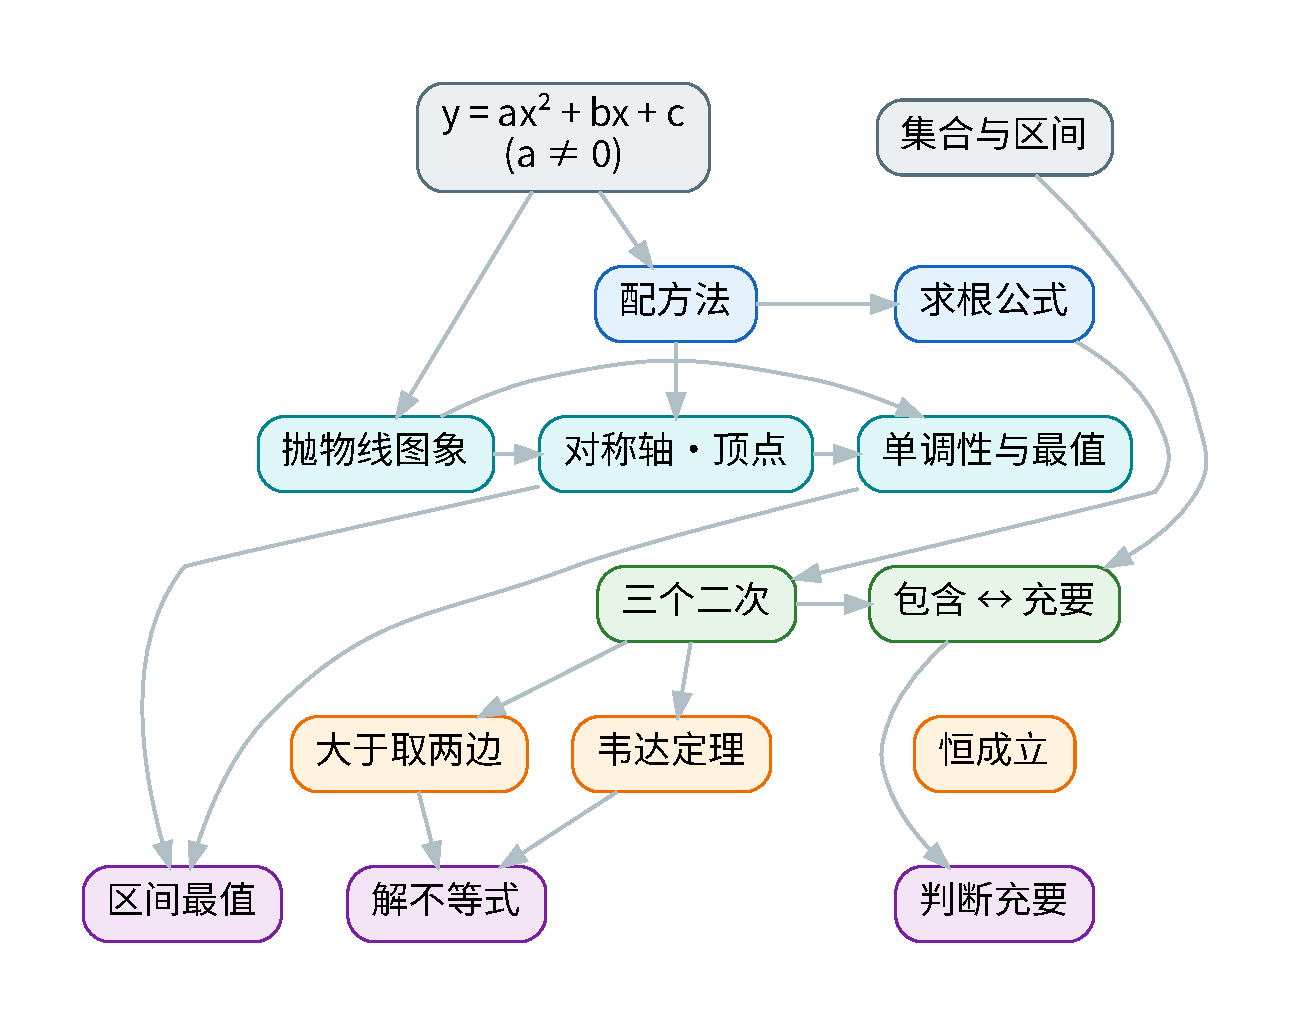
\includegraphics[width=\textwidth]{knowledge.pdf}
  \caption{一元二次函数的知识图谱}
\end{figure}

\section{六层结构说明}

\begin{enumerate}
  \item \key{事实层}：定义、符号、图象。这一层没有技巧，靠准确记忆。
  \item \key{操作层}：配方法、求根公式、解不等式的步骤。这一层靠动手练。
  \item \key{性质层}：开口、对称轴、顶点、单调性、最值。这一层靠看图总结。
  \item \key{关系层}：三个二次的统一、集合包含与充分必要条件的对应。这一层靠讲道理。
  \item \key{结论层}：韦达定理、口诀、恒成立条件。这一层靠会用。
  \item \key{策略层}：解题流程图。这一层靠照做。
\end{enumerate}

\section{学习建议}

基础较弱的同学，建议按下面的顺序过关：

\begin{enumerate}
  \item 先过\key{事实层}：能默写定义、说出符号含义；
  \item 再过\key{操作层}：配方、解方程各练熟；
  \item 然后过\key{性质层}：给一个解析式，能画出草图并说出性质；
  \item 最后再碰\key{结论层}：每条结论都要能说出它是从哪一层推出来的。
\end{enumerate}

\key{不要跳层。} 结论背得再熟，如果不知道它从哪来，换个条件就不会用。

\section{二级结论卡片}

二级结论是从定义和性质推出来的、使用频率高的结果。
下面每张卡片包含五栏：结论、推导、适用条件、易错点、配套练习。

\begin{table}[htbp]
\centering
\small
\setlength{\tabcolsep}{3pt}
\renewcommand{\arraystretch}{1.5}
\begin{tabular}{p{2.6cm}p{4.5cm}p{1.8cm}p{2.5cm}p{0.9cm}}
\toprule
\key{结论} & \key{推导} & \key{适用条件} & \key{易错点} & \key{层级} \\
\midrule
顶点坐标
$\left(-\dfrac{b}{2a},\dfrac{4ac-b^2}{4a}\right)$
& 对 $ax^2+bx+c$ 配方
& $a\neq0$ & 符号写错；忘记 $a\neq0$ & 一级 \\
\addlinespace
判别式
$\Delta=b^2-4ac$
& 由求根公式中根号内的部分得到
& 方程必须是一元二次 & 只记公式，不会判断根的个数 & 一级 \\
\addlinespace
韦达定理
$x_1+x_2=-\dfrac{b}{a}$，
$x_1x_2=\dfrac{c}{a}$
& 由求根公式相加、相乘得到
& $\Delta\geq0$ & 忽略 $\Delta\geq0$ 的前提 & 二级 \\
\addlinespace
大于取两边，小于取中间
& 由图象在 $x$ 轴上方 / 下方得到
& $a>0$ 且已因式分解 & $a<0$ 时不化正就用，方向错 & 二级 \\
\addlinespace
左同右异
（对称轴在 $y$ 轴左，$a,b$ 同号；在右，异号）
& 由 $x=-\dfrac{b}{2a}$ 与 $0$ 比较得到
& $a\neq0$ & 只记口诀，不会推导 & 三级 \\
\addlinespace
恒成立条件
$ax^2+bx+c>0$ 恒成立
$\iff a>0$ 且 $\Delta<0$
& 由「图象全部在 $x$ 轴上方」得到
& 二次项系数含参时需讨论 & 漏掉 $a=0$ 的讨论 & 二级 \\
\addlinespace
根的分布
（两根都在区间内）
& 用对称轴位置、端点函数值符号、$\Delta$ 联立
& 需分类讨论 & 条件列不全，漏掉 $\Delta$ & 三级 \\
\bottomrule
\end{tabular}
\caption{常见二级结论卡片}
\end{table}

\section{使用建议}

\begin{itemize}
  \item \key{一级}：必须能独立推导，且能讲清楚每一步的依据；
  \item \key{二级}：记住形式，会用；知道它是从哪一层推出来的；
  \item \key{三级}：看懂即可，不要求默写，遇到时知道有这个工具。
\end{itemize}

\section{复习节奏}

同一条结论至少要在三个地方出现：

\begin{enumerate}
  \item 新授课：推导它（第一次）；
  \item 基础练习：直接套用它（第二次）；
  \item 综合题：在变化的条件下辨认它（第三次）。
\end{enumerate}

\section{解题流程图（补充说明）}

下面几张流程图是\key{补充材料}，供做题时对照使用，不单独作为知识点讲授。

\subsection{解一元二次不等式}

\begin{figure}[htbp]
  \centering
  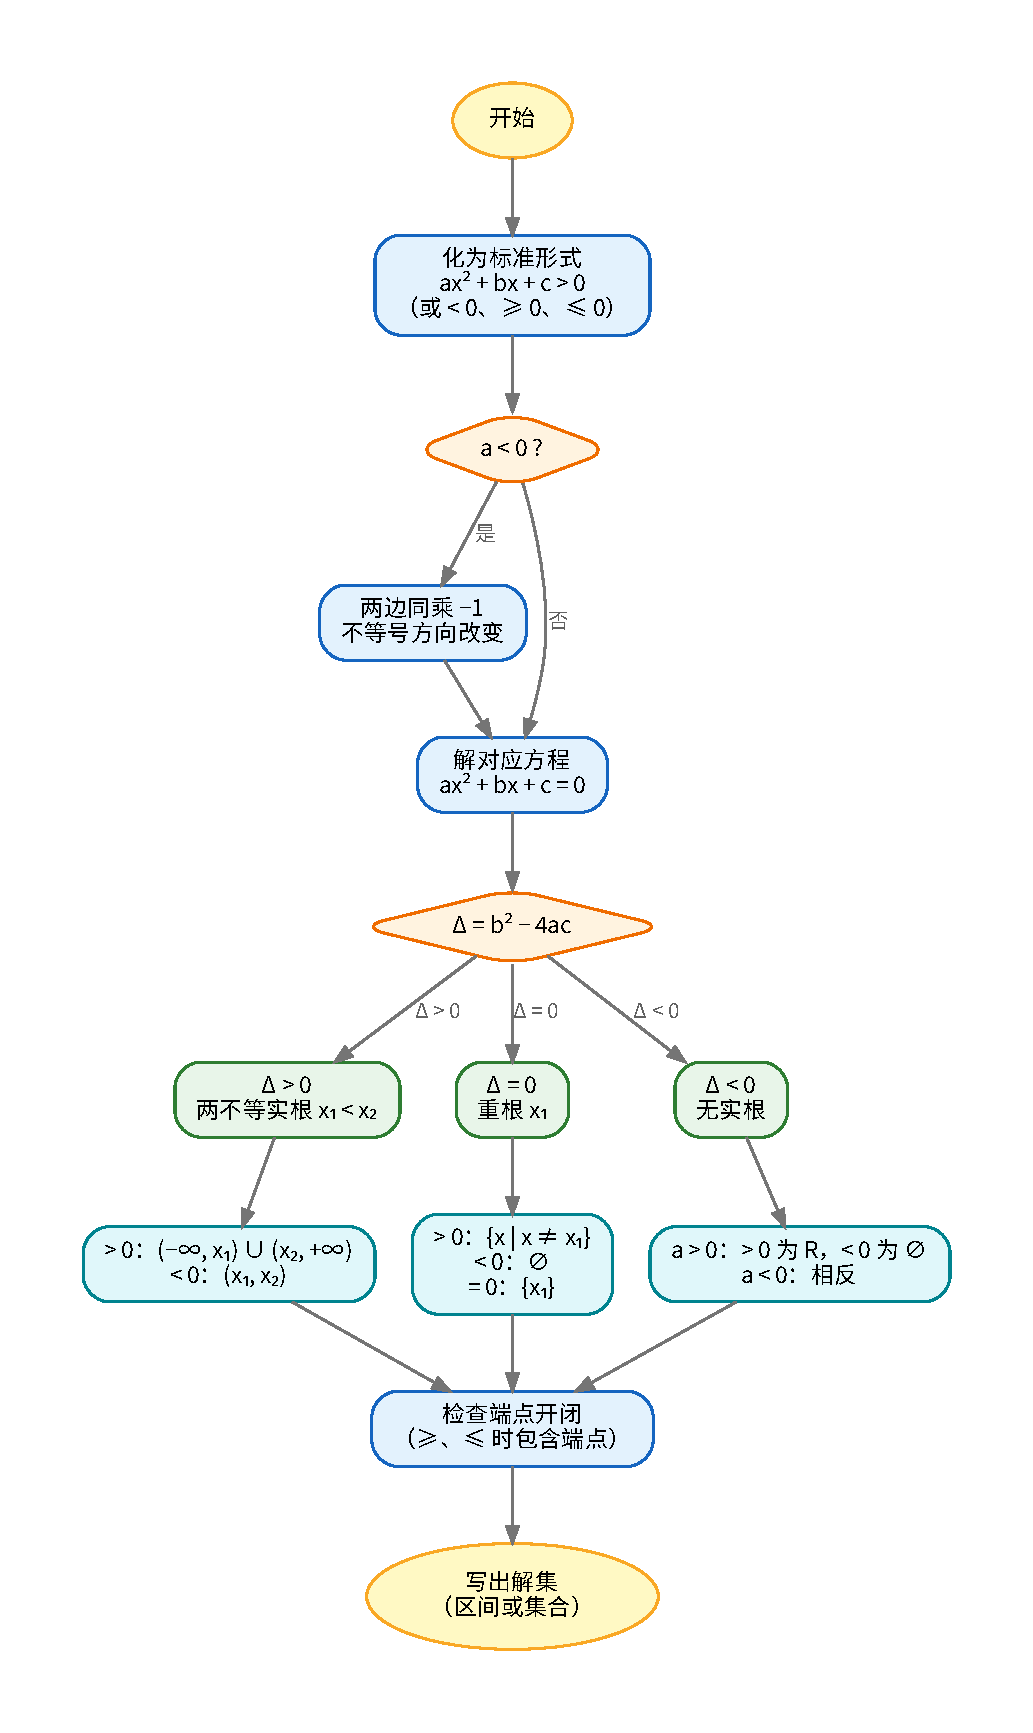
\includegraphics[width=0.60\textwidth]{flow-inequality.pdf}
  \caption{解一元二次不等式的完整流程}
\end{figure}

\key{一句话记忆}：先化正，再求根，后定区间，最后查端点。

\subsection{判断充分条件与必要条件}

\begin{figure}[htbp]
  \centering
  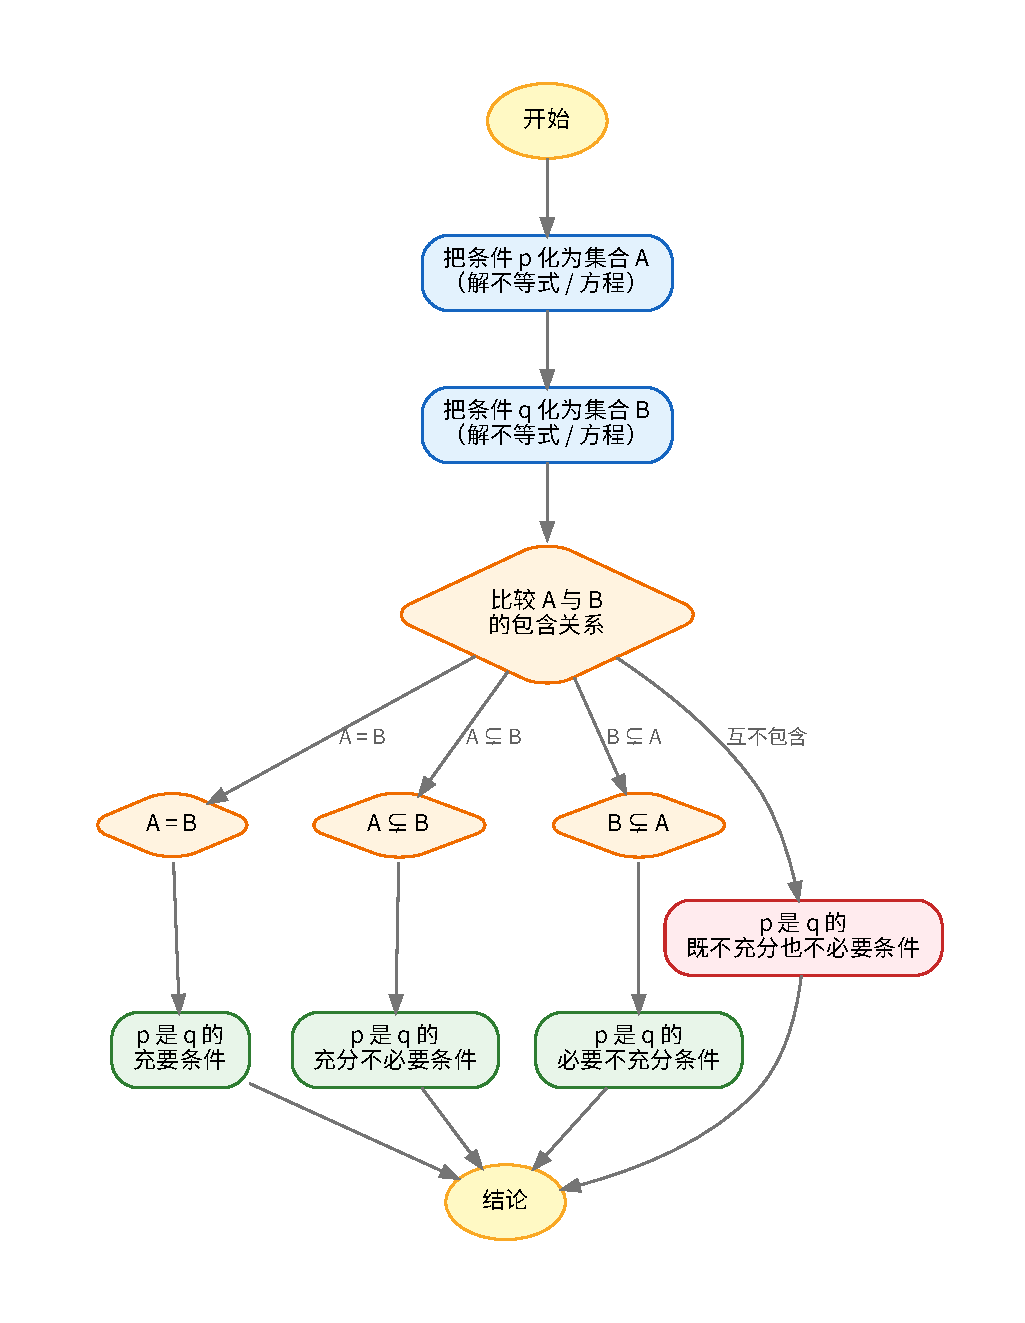
\includegraphics[width=0.60\textwidth]{flow-condition.pdf}
  \caption{用集合包含关系判断充分必要条件}
\end{figure}

\key{一句话记忆}：小范围推大范围，范围相等即充要。

\subsection{求二次函数在区间上的最值}

\begin{figure}[htbp]
  \centering
  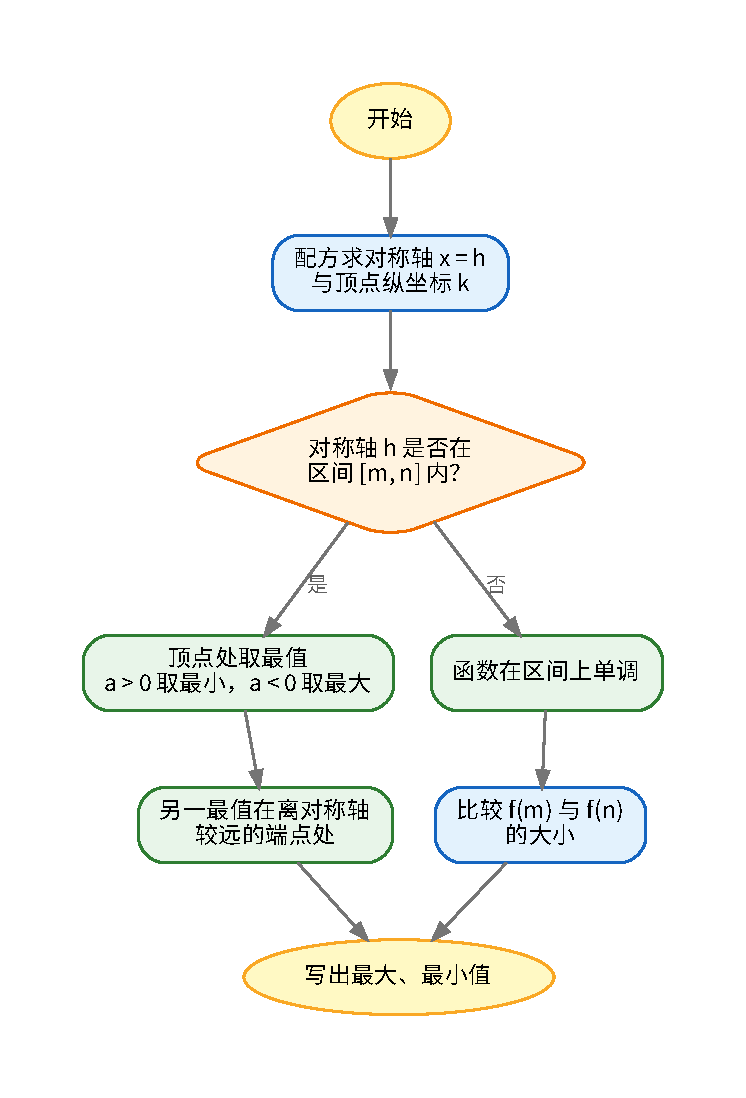
\includegraphics[width=0.60\textwidth]{flow-extreme.pdf}
  \caption{区间最值的分类讨论流程}
\end{figure}

\key{一句话记忆}：先看对称轴在不在区间内，在则顶点，不在则端点。

\subsection{解指数、对数不等式}

\begin{figure}[htbp]
  \centering
  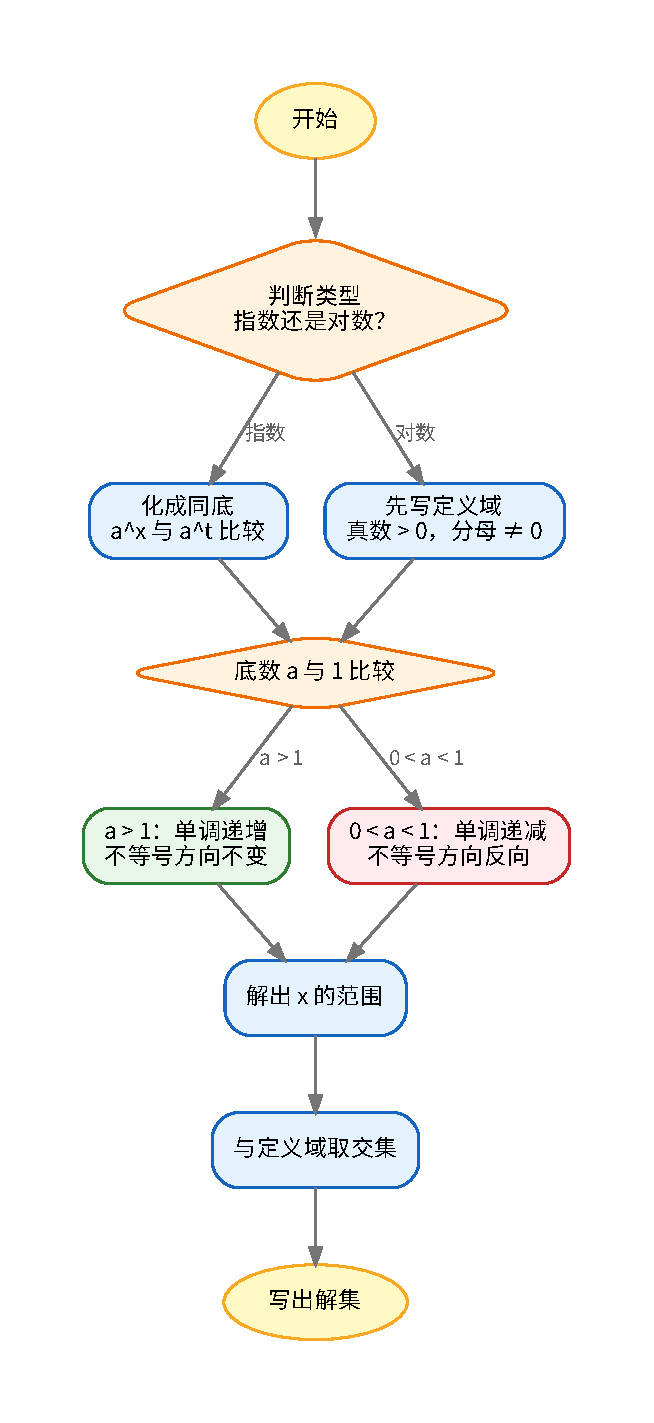
\includegraphics[width=0.62\textwidth]{flow-exp-log.pdf}
  \caption{解指数与对数不等式的流程}
\end{figure}

\key{一句话记忆}：先化同底，再看底数与 $1$ 的大小；对数别忘定义域。

\subsection{求 $y=A\sin(\omega x+\varphi)+b$ 的性质}

\begin{figure}[htbp]
  \centering
  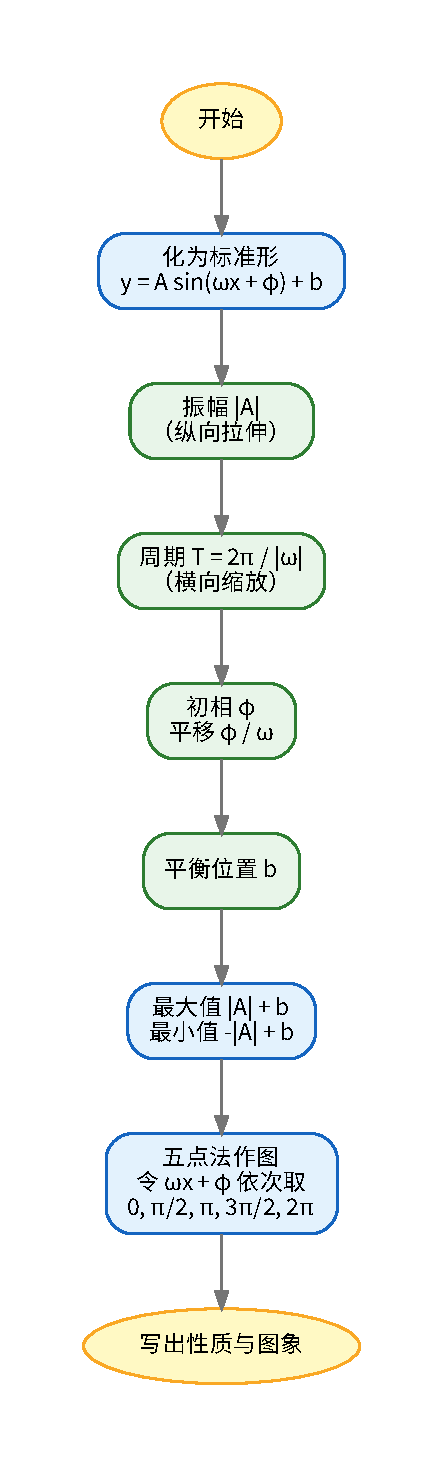
\includegraphics[width=0.56\textwidth]{flow-trig.pdf}
  \caption{由三个参数到图象与性质的流程}
\end{figure}

\key{一句话记忆}：$A$ 管高低，$\omega$ 管快慢，$\varphi$ 管左右，$b$ 管上下平移。

\subsection{流程图的用法}

流程图不是用来看的，是用来\key{照着做}的。建议：

\begin{enumerate}
  \item 做题时把流程图放在手边，一步一步对照；
  \item 每做一步，在题目上标出对应的是流程图中的哪一步；
  \item 做完十道题以后，尝试不对照流程图独立完成；
  \item 期末复习时，把流程图默写一遍。
\end{enumerate}


\end{document}
